\chapter{Market Data: Stock Price Analysis}
\label{ch:stocks}

\begin{companioncode}{qf-03-stocks}
Code: \texttt{crates/qf-03-stocks/}\\
Dependencies: \crate{qf-common}\\
Run: \texttt{cargo run -p qf-03-stocks --example stock\_analysis}
\end{companioncode}

\section{Learning Objectives}

This chapter introduces the fundamental data structure of quantitative finance:
\textbf{OHLCV} (Open, High, Low, Close, Volume) market data. We learn:

\begin{itemize}
    \item OHLCV data structure and its significance
    \item Candlestick anatomy---body, shadows, and what they reveal
    \item Basic market statistics (range, volume, price change)
    \item Moving averages: SMA and EMA
    \item The \texttt{TimeSeries} trait for generic operations
\end{itemize}

\begin{keyinsight}
OHLCV data is the foundation of all quantitative analysis. Every strategy,
every backtest, every indicator starts here. Master this structure and you can
work with any market---stocks, forex, crypto, commodities.
\end{keyinsight}

\section{Introduction: What is OHLCV?}

\marginnote{%
\textbf{OHLCV}\\[0.3em]
Open, High, Low, Close, Volume---the five essential data points for any trading
period (day, hour, minute).
}

Every trading period (day, hour, minute) produces five key data points:

\begin{itemize}
    \item \textbf{Open}: First traded price of the period
    \item \textbf{High}: Highest price reached during the period
    \item \textbf{Low}: Lowest price reached during the period
    \item \textbf{Close}: Last traded price of the period
    \item \textbf{Volume}: Total number of shares/contracts traded
\end{itemize}

This data tells a story. The range between high and low shows volatility. The
relationship between open and close shows direction. Volume confirms conviction.

\section{Data Structure}

\subsection{Rust Implementation}

\begin{lstlisting}[language=Rust]
#[derive(Debug, Clone, Deserialize)]
pub struct Ohlcv {
    pub date: String,
    pub open: f64,
    pub high: f64,
    pub low: f64,
    pub close: f64,
    pub volume: u64,
    pub adj_close: Option<f64>,
}
\end{lstlisting}

\marginnote{%
\textbf{Adjusted Close}\\[0.3em]
Accounts for splits and dividends. If a stock splits 2:1, historical closes are
halved so charts remain continuous.
}

\subsection{Data Validation}

OHLCV data has natural constraints that we validate on load:

\begin{itemize}
    \item $\text{low} \leq \text{high}$ (always)
    \item $\text{low} \leq \text{open} \leq \text{high}$
    \item $\text{low} \leq \text{close} \leq \text{high}$
\end{itemize}

\begin{lstlisting}[language=Rust]
// Validate OHLCV relationships
if record.high < record.low {
    return Err(CommonError::ParseError(format!(
        "Row {}: high ({}) < low ({})",
        idx + 2, record.high, record.low
    )));
}
\end{lstlisting}

\section{Candlestick Anatomy}

\marginnote{%
\textbf{Candlestick Parts}\\[0.3em]
Body: $|close - open|$\\
Upper shadow: $high - \max(O, C)$\\
Lower shadow: $\min(O, C) - low$
}

A candlestick visualizes OHLCV data. Understanding its anatomy is essential:

\marginnote{%
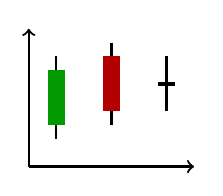
\begin{tikzpicture}[scale=0.35]
\draw[thick, ->] (0,0) -- (6,0);
\draw[thick, ->] (0,0) -- (0,5);
% Bullish
\draw[thick] (1,1) -- (1,4);
\fill[green!60!black] (0.7,1.5) rectangle (1.3,3.5);
% Bearish
\draw[thick] (3,1.5) -- (3,4.5);
\fill[red!70!black] (2.7,2) rectangle (3.3,4);
% Doji
\draw[thick] (5,2) -- (5,4);
\draw[thick, line width=1.5pt] (4.7,3) -- (5.3,3);
\end{tikzpicture}\\[0.3em]
\textbf{Candlesticks}\\
Green: bullish\\
Red: bearish\\
Line: doji
}

\begin{center}
\begin{tabular}{ll}
\toprule
\textbf{Component} & \textbf{Formula} \\
\midrule
Daily Range & $high - low$ \\
Body & $close - open$ \\
Upper Shadow & $high - \max(open, close)$ \\
Lower Shadow & $\min(open, close) - low$ \\
Typical Price & $(high + low + close) / 3$ \\
\bottomrule
\end{tabular}
\end{center}

\subsection{Rust Implementation}

\begin{lstlisting}[language=Rust]
impl Ohlcv {
    /// Daily price range
    pub fn daily_range(&self) -> f64 {
        self.high - self.low
    }

    /// Candle body (positive = bullish)
    pub fn body(&self) -> f64 {
        self.close - self.open
    }

    /// Upper shadow length
    pub fn upper_shadow(&self) -> f64 {
        self.high - self.open.max(self.close)
    }

    /// Lower shadow length
    pub fn lower_shadow(&self) -> f64 {
        self.open.min(self.close) - self.low
    }

    /// True if close > open (green candle)
    pub fn is_bullish(&self) -> bool {
        self.close > self.open
    }

    /// Representative price: (H + L + C) / 3
    pub fn typical_price(&self) -> f64 {
        (self.high + self.low + self.close) / 3.0
    }
}
\end{lstlisting}

\section{Market Statistics}

\subsection{Basic Aggregations}

Given a series of OHLCV records, we compute summary statistics:

\begin{lstlisting}[language=Rust]
/// Average trading volume
pub fn average_volume(data: &[Ohlcv]) -> f64 {
    if data.is_empty() { return 0.0; }
    let sum: u64 = data.iter().map(|o| o.volume).sum();
    sum as f64 / data.len() as f64
}

/// Price change: (last - first) / first
pub fn price_change(data: &[Ohlcv]) -> f64 {
    if data.len() < 2 { return 0.0; }
    let first = data[0].close;
    let last = data[data.len() - 1].close;
    (last - first) / first
}

/// Highest high across all records
pub fn highest_high(data: &[Ohlcv]) -> f64 {
    data.iter().map(|o| o.high).fold(f64::NEG_INFINITY, f64::max)
}

/// Lowest low across all records
pub fn lowest_low(data: &[Ohlcv]) -> f64 {
    data.iter().map(|o| o.low).fold(f64::INFINITY, f64::min)
}
\end{lstlisting}

\marginnote{%
\textbf{Functional Style}\\[0.3em]
Note the use of \texttt{iter()}, \texttt{map()}, \texttt{fold()}---Rust's
functional combinators make statistical computations elegant.
}

\section{Moving Averages}

\subsection{Simple Moving Average (SMA)}

The SMA is the arithmetic mean of the last $n$ prices:

\marginnote{%
\textbf{SMA Formula}\\[0.5em]
$\text{SMA}_t = \dfrac{1}{n}\sum_{i=0}^{n-1} P_{t-i}$\\[0.5em]
where $n$ is the period.
}

\[
\text{SMA}_t = \frac{1}{n}\sum_{i=0}^{n-1} P_{t-i}
\]

\begin{lstlisting}[language=Rust]
pub fn sma(prices: &[f64], period: usize) -> Vec<f64> {
    if period == 0 || period > prices.len() {
        return Vec::new();
    }

    let mut result = Vec::with_capacity(prices.len() - period + 1);

    for i in 0..=(prices.len() - period) {
        let window = &prices[i..i + period];
        let sum: f64 = window.iter().sum();
        result.push(sum / period as f64);
    }

    result
}
\end{lstlisting}

\subsection{Exponential Moving Average (EMA)}

The EMA gives more weight to recent prices, making it more responsive:

\marginnote{%
\textbf{EMA Formula}\\[0.5em]
$\text{EMA}_t = \alpha \cdot P_t + (1-\alpha) \cdot \text{EMA}_{t-1}$\\[0.5em]
$\alpha = \dfrac{2}{n+1}$
}

\[
\text{EMA}_t = \alpha \cdot P_t + (1 - \alpha) \cdot \text{EMA}_{t-1}
\]

where $\alpha = \frac{2}{n+1}$ is the smoothing factor.

\begin{lstlisting}[language=Rust]
pub fn ema(prices: &[f64], period: usize) -> Vec<f64> {
    if period == 0 || prices.is_empty() {
        return Vec::new();
    }

    let alpha = 2.0 / (period + 1) as f64;
    let mut result = Vec::with_capacity(prices.len());

    // Initialize with first price
    result.push(prices[0]);

    // Recursive formula
    for i in 1..prices.len() {
        let prev_ema = result[i - 1];
        let current_ema = alpha * prices[i] + (1.0 - alpha) * prev_ema;
        result.push(current_ema);
    }

    result
}
\end{lstlisting}

\subsection{SMA vs EMA}

\begin{center}
\begin{tabular}{lcc}
\toprule
\textbf{Property} & \textbf{SMA} & \textbf{EMA} \\
\midrule
Weighting & Equal & Exponential \\
Responsiveness & Slower & Faster \\
Lag & More & Less \\
Smoothness & Smoother & Noisier \\
Computation & Simple & Recursive \\
\bottomrule
\end{tabular}
\end{center}

\begin{keyinsight}
SMA is a \emph{lagging} indicator---it tells you what already happened. EMA
reacts faster but can give false signals. Traders often use both: short-term
EMA for entries, long-term SMA for trend confirmation.
\end{keyinsight}

\section{TimeSeries Trait}

Following our trait-based architecture, we define a generic interface:

\begin{lstlisting}[language=Rust]
pub trait TimeSeries {
    fn len(&self) -> usize;
    fn is_empty(&self) -> bool;
    fn closes(&self) -> Vec<f64>;
    fn volumes(&self) -> Vec<u64>;
}

impl TimeSeries for Vec<Ohlcv> {
    fn len(&self) -> usize { self.len() }
    fn is_empty(&self) -> bool { self.is_empty() }

    fn closes(&self) -> Vec<f64> {
        self.iter().map(|o| o.close).collect()
    }

    fn volumes(&self) -> Vec<u64> {
        self.iter().map(|o| o.volume).collect()
    }
}
\end{lstlisting}

\marginnote{%
\textbf{Trait Benefits}\\[0.3em]
The \texttt{TimeSeries} trait allows functions to work with any data source
that can provide price/volume sequences.
}

This enables generic functions that work with any \texttt{TimeSeries}:

\begin{lstlisting}[language=Rust]
fn analyze<T: TimeSeries>(data: &T) -> Report {
    let closes = data.closes();
    let sma_20 = sma(&closes, 20);
    let sma_50 = sma(&closes, 50);
    // ...
}
\end{lstlisting}

\section{Golden and Death Crosses}

A classic trading signal using moving averages:

\begin{itemize}
    \item \textbf{Golden Cross}: Short-term MA crosses \emph{above} long-term MA
      (bullish signal)
    \item \textbf{Death Cross}: Short-term MA crosses \emph{below} long-term MA
      (bearish signal)
\end{itemize}

\begin{lstlisting}[language=Rust]
fn find_crossovers(short_ma: &[f64], long_ma: &[f64]) -> Vec<(usize, bool)> {
    let mut crossovers = Vec::new();

    for i in 1..short_ma.len().min(long_ma.len()) {
        let prev_above = short_ma[i-1] > long_ma[i-1];
        let curr_above = short_ma[i] > long_ma[i];

        if !prev_above && curr_above {
            crossovers.push((i, true));  // Golden cross
        } else if prev_above && !curr_above {
            crossovers.push((i, false)); // Death cross
        }
    }

    crossovers
}
\end{lstlisting}

\section{Results and Analysis}

\subsection{Example Output}

\begin{lstlisting}[language=bash]
$ cargo run -p qf-03-stocks --example stock_analysis
Loading OHLCV data from data/spy.csv...
Loaded 252 trading days

Statistics:
  Average Volume: 85,432,100
  Price Change: +12.5%
  Highest High: $485.32
  Lowest Low: $410.15
  Average Daily Range: $5.23

Moving Averages:
  SMA(20) latest: $472.15
  SMA(50) latest: $465.80
  EMA(20) latest: $474.22

Crossovers (last 12 months):
  Day 45: Golden Cross (bullish)
  Day 128: Death Cross (bearish)
  Day 201: Golden Cross (bullish)
\end{lstlisting}

\section{Exercises}

\begin{enumerate}
    \item \textbf{Candlestick Patterns}: Implement detection for ``doji''
      (open $\approx$ close) and ``hammer'' (small body, long lower shadow).

    \item \textbf{Volume Analysis}: Add \func{volume\_ma} that computes moving
      average of volume. Flag days where volume exceeds 2x the average.

    \item \textbf{Bollinger Bands}: Implement Bollinger Bands: SMA $\pm$ 2
      standard deviations. This requires computing rolling standard deviation.

    \item \textbf{MACD}: Implement the MACD indicator: EMA(12) - EMA(26), with
      a 9-period signal line.

    \item \textbf{Backtest}: Using SMA crossover signals, simulate a simple
      strategy: buy on golden cross, sell on death cross. Track P\&L.
\end{enumerate}

\section{Key Takeaways}

\begin{itemize}
    \item \textbf{OHLCV} is the atomic unit of market data
    \item \textbf{Candlesticks} encode price action: body shows direction,
      shadows show rejection
    \item \textbf{SMA} averages equally; \textbf{EMA} weights recent prices
    \item \textbf{Crossovers} generate trading signals (but beware of lag!)
    \item \textbf{TimeSeries trait} enables generic, reusable analysis code
\end{itemize}

\vspace{1em}
\noindent\textbf{Next chapter}: Returns and volatility---the foundation of risk
measurement and portfolio theory.
